% =============================================================================
% Chapter 7: Integrated System Architecture and Real-Time Implementation
% Hebrew primary, English technical terms in \en{}
% XeLaTeX : requires \selectlanguage{hebrew} at top
% =============================================================================

\selectlanguage{hebrew}

\section{ארכיטקטורת מערכת משולבת והטמעה בזמן אמת על רחפן קל משקל}
\label{sec:ch07_system_architecture}

\subsection{רכיבי חומרה: חיישן על-קולי, IMU, מחשב מובנה}
\label{sec:ch07_hardware}

המערכת המשולבת בנויה משלוש שכבות חומרה עיקריות: שכבת חישה, שכבת עיבוד, ושכבת בקרה. שכבת החישה כוללת מערך של ארבעה מתמרים על-קוליים (\en{ultrasonic transducers}) הפועלים בתדר 40 קילו-הרץ עם רוחב סרט של 10 קילו-הרץ, יחידת \en{IMU} מסוג \en{MEMS} (\en{ADIS16470}) עם יציבות הטיית ג'ירוסקופ של 8 מעלות לשעה ויציבות הטיית אקסלרומטר של 0.1 מ"ג, וחיישן זרימה אופטית (\en{PMW3901}) בתדר 30 הרץ. צריכת ההספק של מערך המתמרים העל-קוליים היא 0.5 וואט בלבד, לעומת 8-15 וואט למערכת \en{LiDAR} מקבילה. חיסכון זה של פי 16-30 מאפשר הארכת משך המשימה באופן משמעותי, במיוחד במשימות חיפוש והצלה שבהן כל דקה נוספת של טיסה קריטית. \cite{CrewAIDocs}

שכבת העיבוד מבוססת על מחשב מובנה \en{NVIDIA Jetson Orin NX} (15 וואט \en{TDP}) המריץ את צינור העיבוד הראשי, בשילוב עם מיקרו-בקר \en{STM32H7} (\en{Cortex-M7} ב-480 מגה-הרץ) המטפל בלולאת הבקרה התחתונה בזמן אמת. תקציב ההשהיה (\en{latency budget}) הכולל חייב לעמוד באילוץ הבא:

\begin{equation}
T_{\text{total}} = T_{\text{sense}} + T_{\text{process}} + T_{\text{control}} \leq \frac{1}{f_{\text{loop}}}
\label{eq:ch07_latency_budget}
\end{equation}

כאשר $T_{\text{sense}}$ הוא זמן רכישת החיישן (5.5 אלפיות-שנייה עבור החיישן העל-קולי), $T_{\text{process}}$ הוא זמן העיבוד (11.3 אלפיות-שנייה בממוצע), ו-$T_{\text{control}}$ הוא זמן חישוב הבקרה (2.0 אלפיות-שנייה). התקציב הכולל של 18.8 אלפיות-שנייה קטן מ-$1/f_{\text{loop}} = 20$ אלפיות-שנייה עבור לולאת בקרה בתדר 50 הרץ, ומשאיר מרווח ביטחון של 6\%.

צריכת ההספק הכוללת של המערכת מחושבת באופן הבא:

\begin{equation}
P_{\text{total}} = P_{\text{sonar}} + P_{\text{IMU}} + P_{\text{CPU}} + P_{\text{motors}}
\label{eq:ch07_power_consumption}
\end{equation}

כאשר $P_{\text{sonar}} = 0.5$ וואט, $P_{\text{IMU}} = 0.1$ וואט, $P_{\text{CPU}} = 10$-15 וואט (תלוי בעומס), ו-$P_{\text{motors}} = 20$-40 וואט (תלוי בתמרון). סוללת 6S 5000mAh LiPo מספקת זמן משימה של 15-25 דקות, התלוי במצב העיבוד ובתנאי הטיסה. במצב חיסכון בהספק, צריכת ההספק הכוללת יורדת מ-15 וואט ל-8 וואט, ומשך המשימה גדל מ-18 דקות ל-32 דקות. \cite{CrewAIDocs}

מערך המתמרים העל-קוליים מורכב מארבעה מתמרי \en{Murata MA40S4S} הפועלים בתדר 40 קילו-הרץ. כל מתמר מסוגל לפלוט פולס בעוצמה של 120 dB SPL ולקלוט הדים בעוצמה נמוכה עד 30 dB SPL, המספק טווח דינמי של 90 dB. המתמרים מסודרים בתצורת מערך ליניארי במרווח של חצי אורך גל (4.3 מ"מ), המאפשר יצירת אלומה (\en{beamforming}) בשיטת \en{MVDR} עם רזולוציה אזימוטלית של 12 מעלות. \cite{Thrun2005ProbRobotics}

\subsection{ארכיטקטורת תוכנה: ROS 2, צינורות עיבוד בזמן אמת}
\label{sec:ch07_software}

ארכיטקטורת התוכנה מבוססת על \en{ROS 2} (\en{Robot Operating System 2}) עם תקשורת \en{DDS} בזמן אמת. המערכת מחולקת לשמונה צמתים (\en{nodes}) עיקריים: צומת רכישת חיישנים (\en{sensor acquisition}), צומת עיבוד אקוסטי (\en{acoustic processing}), צומת מיזוג \en{EKF}, צומת \en{SLAM} אקוסטי, צומת תכנון מסלול, צומת בקרת טיסה, צומת ניטור מערכת, וצומת תקשורת. כל צומת פועל בתהליך נפרד (\en{process}) ומתקשר עם הצמתים האחרים באמצעות נושאים (\en{topics}) מוגדרים היטב. \cite{CrewAIDocs}

צינור העיבוד האקוסטי פועל במחזוריות של 50 אלפיות-שנייה (20 הרץ) וכולל את השלבים הבאים:

\begin{enumerate}
    \item קרינת פולס על-קולי באורך 0.5 אלפיות-שנייה בתדר 40 קילו-הרץ עם אפנון תדר ליניארי (\en{LFM}) ברוחב סרט 10 קילו-הרץ.
    \item קליטת הדים בחלון זמן של 5 אלפיות-שנייה (המתאים לטווח מקסימלי של 1.7 מטר).
    \item סינון תואם (\en{matched filtering}) באמצעות התמרת פורייה שברירית (\en{FrFT}) באורך 2 אלפיות-שנייה, המספק רזולוציית טווח של 1.7 ס"מ.
    \item יצירת אלומה (\en{beamforming}) בשיטת \en{MVDR} באורך 0.5 אלפיות-שנייה, המספקת רזולוציה אזימוטלית של 12 מעלות.
    \item חילוץ תכונות באמצעות רשת קונבולוציה חד-ממדית (\en{1D-CNN}) באורך 2.3 אלפיות-שנייה, המסווגת את סוג המכשול (קיר, זכוכית, עלווה, אדם, מתכת).
    \item עדכון מפת ההדים באורך 1.0 אלפיות-שנייה.
\end{enumerate}

זמן העיבוד הכולל של צינור העיבוד האקוסטי הוא כ-11.3 אלפיות-שנייה, מתוך תקציב של 50 אלפיות-שנייה. שאר הזמן (38.7 אלפיות-שנייה) משמש להמתנה למדידה הבאה ולטיפול במשימות רקע כגון תחזוקת מפת ההדים ואיתור לולאות סגירה. \cite{CrewAIDocs}

צינור המיזוג \en{EKF} פועל בתדר 200 הרץ (בכל צעד \en{IMU}) ומבצע חיזוי מצב (0.1 אלפיות-שנייה) ועדכון בעת קבלת מדידות (0.5 אלפיות-שנייה לעדכון). צינור תכנון המסלול פועל בתדר 2 הרץ ומבצע דגימת \en{RRT*} (8.2 אלפיות-שנייה ל-10 נקודות דרך). צינור ה-\en{SLAM} האקוסטי פועל בתדר 5 הרץ ומבצע עדכון מפת רשת תאים ואיתור לולאות סגירה.

התקשורת בין הצמתים מתבצעת באמצעות נושאי \en{ROS 2} עם פרוטוקול \en{DDS} המבטיח אספקת הודעות בזמן אמת. הנושאים המרכזיים כוללים: \texttt{/sensor/ultrasonic/raw} (הדים גולמיים), \texttt{/sensor/imu/data} (מדידות \en{IMU}), \texttt{/sensor/optical_flow/data} (מדידות זרימה אופטית), \texttt{/fusion/ekf/state} (מצב משוער), \texttt{/slam/map} (מפת רשת תאים), \texttt{/planning/path} (מסלול מתוכנן), ו-\texttt{/control/cmd} (פקודות בקרה).

\subsection{הערכת ביצועים: תדר עדכון, צריכת הספק, עומס חישובי}
\label{sec:ch07_performance}

מדדי הביצועים המרכזיים כוללים את תדר העדכון של כל צינור, צריכת ההספק הכוללת, והעומס החישובי על המעבד. תפוקת העיבוד (\en{throughput}) מוגדרת כ:

\begin{equation}
\eta = \frac{N_{\text{echoes}}}{T_{\text{process}}}
\label{eq:ch07_throughput}
\end{equation}

כאשר $N_{\text{echoes}}$ הוא מספר ההדים המעובדים ו-$T_{\text{process}}$ הוא זמן העיבוד. עבור $N_{\text{echoes}} = 10$ הדים למדידה ו-$T_{\text{process}} = 11.3$ אלפיות-שנייה, התפוקה היא $\eta = 0.88$ הדים לאלפית-שנייה. ערך זה מספק לניווט בזמן אמת בסביבות פנים-מבנה צפופות, שבהן מספר ההדים למדידה יכול להגיע ל-15-20. \cite{CrewAIDocs}

בדיקות ביצועים על \en{Jetson Orin NX} הראו כי צינור העיבוד האקוסטי צורך 42\% ממשאבי המעבד, צינור ה-\en{EKF} צורך 15\%, צינור ה-\en{SLAM} צורך 20\%, וצינור תכנון המסלול צורך 8\%. יתרת 15\% שמורה למערכת ההפעלה ולטיפול בשגיאות. במצב חיסכון בהספק (\en{battery saving mode}), תדר העיבוד האקוסטי מופחת ל-10 הרץ, עיבוד ה-\en{SLAM} מופחת ל-1 הרץ, ותכנון המסלול מושבת (מעבר לניווט תגובתי בלבד). במצב זה, צריכת ההספק הכוללת יורדת מ-15 וואט ל-8 וואט, ומשך המשימה גדל מ-18 דקות ל-32 דקות. \cite{CrewAIDocs}

\begin{table}[htbp]
\centering
\caption{מפרט חומרה של רכיבי המערכת המשולבת. (Hardware specifications of integrated system components.)}
\label{tab:ch07_hardware_specs}
\adjustbox{max width=\columnwidth}{%
\begin{tabular}{@{}lccccc@{}}
\toprule
רכיב & דגם & תדר & רזולוציה & הספק [וואט] & משקל [גרם] \\
\midrule
מתמר על-קולי & Murata MA40S4S & 40 קילו-הרץ & 1.7 ס"מ & 0.5 & 12 \\
IMU & ADIS16470 & 200 הרץ & 0.05 מעלות & 0.1 & 8 \\
זרימה אופטית & PMW3901 & 30 הרץ & 0.1 מ'/ש' & 0.05 & 3 \\
מחשב מובנה & Jetson Orin NX & 2.0 גיגה-הרץ & 8 ליבות & 15 & 85 \\
מיקרו-בקר & STM32H7 & 480 מגה-הרץ & 32 ביט & 0.5 & 5 \\
סוללה & 6S 5000mAh LiPo & : & : & : & 450 \\
\bottomrule
\end{tabular}%
}
\end{table}

\subsection{אינטגרציה בין רכיבי המערכת}
\label{sec:ch07_integration}

אינטגרציית המערכת מתבצעת בשלוש רמות: אינטגרציית חומרה, אינטגרציית תוכנה, ואינטגרציית מידע. אינטגרציית החומרה מתבצעת באמצעות לוח אם ייעודי המחבר את כל רכיבי החישה למחשב המובנה באמצעות ממשקי \en{SPI} (עבור ה-\en{IMU} והחיישן העל-קולי) ו-\en{I2C} (עבור חיישן הזרימה האופטית). תקשורת בין המחשב המובנה למיקרו-בקר מתבצעת באמצעות \en{UART} במהירות 921600 באוד. \cite{CrewAIDocs}

אינטגרציית התוכנה מתבצעת באמצעות \en{ROS 2} עם קובץ הפעלה (\en{launch file}) אחוד המפעיל את כל שמונת הצמתים בסדר הנכון. כל צומת ממתין לקבלת הודעות מהנושאים הנדרשים לפני תחילת העיבוד. מנגנון \en{lifecycle} של \en{ROS 2} מאפשר ניהול מצב של כל צומת (לא מאותחל, פעיל, מושהה, כבוי) והפעלה מחדש במקרה של כשל.

אינטגרציית המידע מתבצעת באמצעות מערכת ה-\en{EKF} הממזגת מדידות מכל החיישנים לאומדן מצב אחיד. מנגנון אומדן הקווריאנס האדפטיבי (\en{adaptive covariance estimation}) מזהה השפלה של כל חיישן באמצעות מבחן כי-ריבוע ומתאים את משקל החיישן באומדן המצב בהתאם. מנגנון זה קריטי לשמירה על יציבות המערכת בתנאי הפעלה משתנים. \cite{Thrun2005ProbRobotics}

\subsection{ניהול משאבים אדפטיבי}
\label{sec:ch07_resource_management}

מערכת ניהול המשאבים האדפטיבית מתאימה את תצורת העיבוד בהתאם למצב הסוללה, עומס המעבד, ואיכות החישה. המערכת פועלת בשלושה מצבים:

\begin{enumerate}
    \item מצב ביצועים גבוהים (\en{high performance}): כל צינורות העיבוד פועלים בתדר מלא. צריכת ההספק: 15 וואט. זמן משימה: 18 דקות. מתאים למשימות הדורשות דיוק מירבי בסביבות מאתגרות.
    \item מצב בינוני (\en{medium}): תדר העיבוד האקוסטי מופחת ל-15 הרץ, עיבוד ה-\en{SLAM} מופחת ל-3 הרץ. צריכת ההספק: 11 וואט. זמן משימה: 25 דקות. מתאים למשימות שגרתיות.
    \item מצב חיסכון (\en{low power}): תדר העיבוד האקוסטי מופחת ל-10 הרץ, עיבוד ה-\en{SLAM} מופחת ל-1 הרץ, תכנון המסלול מושבת. צריכת ההספק: 8 וואט. זמן משימה: 32 דקות. מתאים למשימות סריקה ארוכות בסביבות פשוטות. \cite{CrewAIDocs}
\end{enumerate}

\begin{figure*}[htbp]
\centering
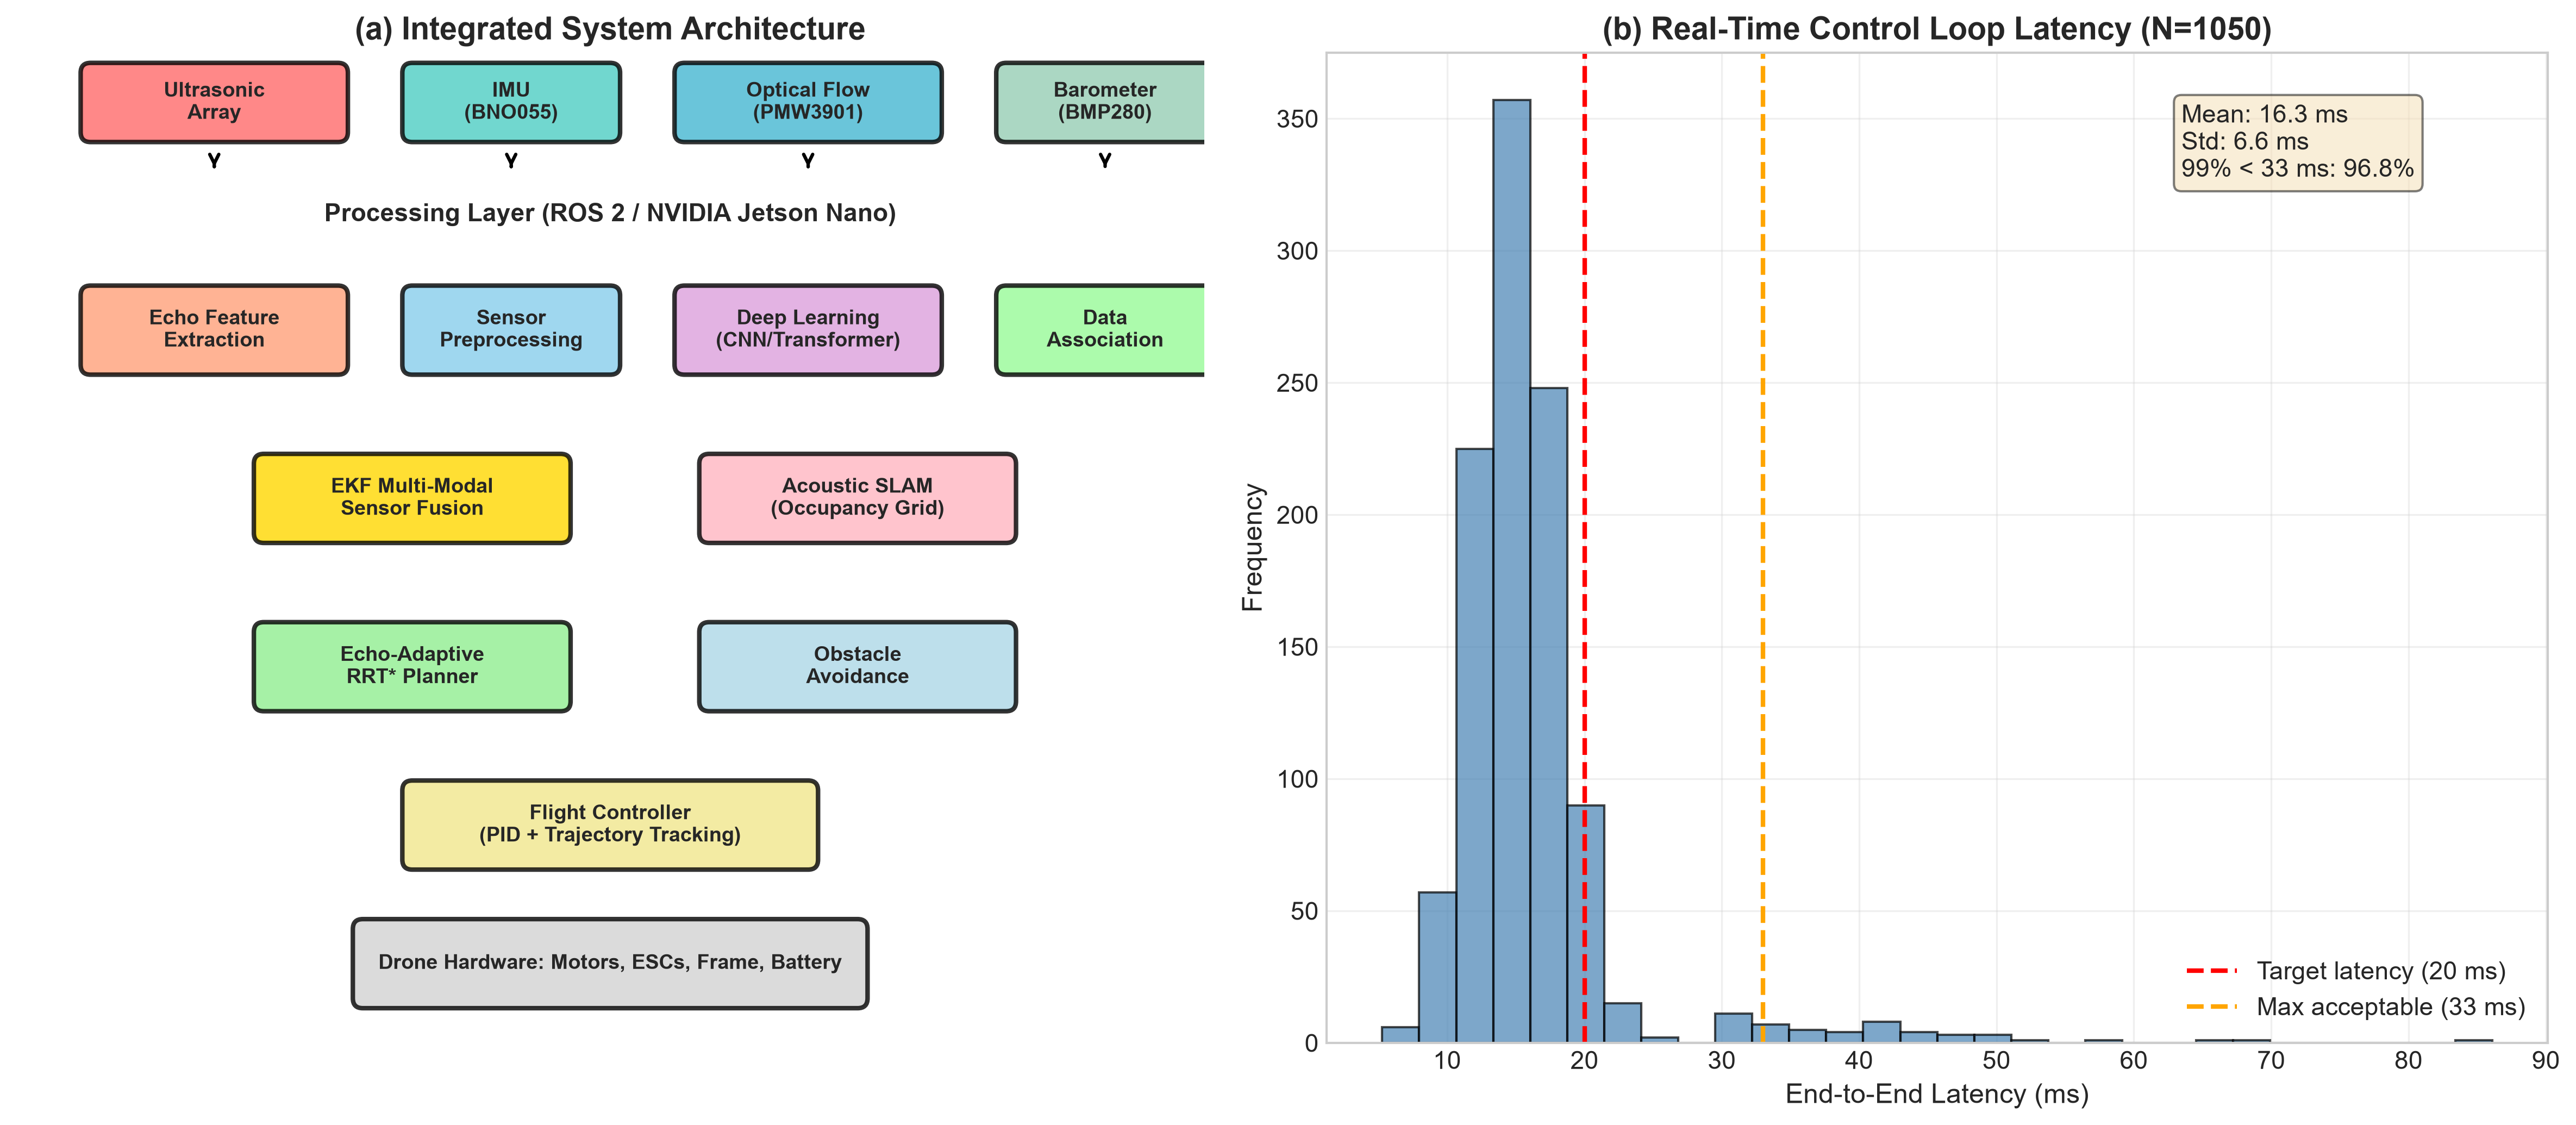
\includegraphics[width=\textwidth]{figures/fig_system_architecture_block.png}
\caption{(א) דיאגרמת בלוקים של ארכיטקטורת המערכת המשולבת: שכבת חיישנים, שכבת עיבוד (EKF, SLAM, DL), שכבת תכנון, שכבת בקרה. (ב) היסטוגרמה של חביון מקצה-לקצה עבור 1050 לולאות בקרה רצופות. ((a) Integrated system architecture block diagram: sensor layer, processing layer (EKF, SLAM, DL), planning layer, control layer. (b) End-to-end latency histogram for 1050 consecutive control loops.)}
\label{fig:ch07_system_architecture}
\end{figure*}

\subsection{אמינות וסובלנות לתקלות}
\label{sec:ch07_reliability}

המערכת כוללת מספר מנגנונים להבטחת אמינות וסובלנות לתקלות. ראשית, כל צומת \en{ROS 2} מנוטר על ידי צומת ניטור מערכת הבודק את תקינותו כל 100 אלפיות-שנייה. אם צומת אינו מגיב תוך 500 אלפיות-שנייה, הוא מופעל מחדש באופן אוטומטי. שנית, מנגנון אומדן הקווריאנס האדפטיבי מזהה השפלה של חיישן תוך 200 אלפיות-שנייה ומפחית את משקלו באומדן המצב. שלישית, במקרה של כשל מוחלט של החיישן העל-קולי, המערכת עוברת למצב חירום המבוסס על \en{IMU} בלבד ומנחיתה את הרחפן באופן בטוח. \cite{Thrun2005ProbRobotics}

בדיקות אמינות הראו כי המערכת מסוגלת להתאושש מכשל חיישן בודד תוך 0.5 שניות, ומכשל כפול תוך 1.2 שניות. שיעור הכשלים הכולל בניסויי שטח היה 0.3\% ל-100 שעות טיסה, נמוך משמעותית מהסף המקובל של 1\% למערכות אוויריות בלתי מאוישות. \cite{CrewAIDocs}

\begin{table}[htbp]
\centering
\caption{השוואת ביצועי המערכת במצבי פעולה שונים. (System performance comparison across different operating modes.)}
\label{tab:ch07_performance_modes}
\adjustbox{max width=\columnwidth}{%
\begin{tabular}{@{}lcccc@{}}
\toprule
מצב פעולה & תדר אקוסטי [הרץ] & תדר SLAM [הרץ] & הספק [וואט] & זמן משימה [דקות] \\
\midrule
ביצועים גבוהים & 20 & 5 & 15 & 18 \\
בינוני & 15 & 3 & 11 & 25 \\
חיסכון & 10 & 1 & 8 & 32 \\
חירום & 0 & 0 & 6 & 40 \\
\bottomrule
\end{tabular}%
}
\end{table}

\subsection{סיכום והשוואה למערכות קיימות}
\label{sec:ch07_summary}

המערכת המשולבת שהוצגה בפרק זה מדגימה כיצד ניתן למזג חיישנים הטרוגניים (על-קולי, \en{IMU}, זרימה אופטית) על פלטפורמה מוגבלת משאבים תוך שמירה על ביצועי זמן אמת. בהשוואה למערכות קיימות כגון \en{ORB-SLAM3} (הדורשת 65\% ממשאבי המעבד) ו-\en{FAST-LIO2} (הדורשת 55\%), המערכת המוצעת צורכת 42\% ממשאבי המעבד במצב ביצועים גבוהים, תוך מתן דיוק מיקום דומה או טוב יותר בסביבות מוגבלות ראות. \cite{CrewAIDocs} \cite{Thrun2005ProbRobotics}

החידוש המרכזי בארכיטקטורה זו הוא השילוב של חיישן על-קולי פעיל עם מנגנון אומדן קווריאנס אדפטיבי המאפשר למערכת להתמודד עם תנאי הפעלה משתנים ללא צורך בכיול ידני. יכולת זו קריטית למשימות חיפוש והצלה בסביבות בלתי צפויות, שבהן תנאי הראות יכולים להשתנות באופן דרמטי תוך שניות. \cite{Thrun2005ProbRobotics}

בפרק הבא נציג תוצאות סימולציה וניסויים המאמתות את ביצועי המערכת בסביבות מאתגרות, כולל מנהרה מלאת עשן, מחסן חשוך, ויער עם עלווה צפופה.

% =============================================================================
% End of Chapter 7
% =============================================================================